% Arquivo LaTeX de exemplo de dissertação/tese a ser apresentados ?CPG do IME-USP
% 
% Vers? 5: Sex Mar  9 18:05:40 BRT 2012
%
% Cria?o: Jes?s P. Mena-Chalco
% Revis?: Fabio Kon e Paulo Feofiloff
%  
% Obs: Leia previamente o texto do arquivo README.txt

\documentclass[12pt,twoside,a4paper]{book} % utilizando extbook para atender ao modelo do IPT

\usepackage{sectsty}
\allsectionsfont{\Large\bfseries}

% ---------------------------------------------------------------------------- %
% Pacotes 
\usepackage{fontspec}
\setmainfont{Arial} % funciona com windows/mac
%\usepackage{polyglossia}
%\setdefaultlanguage{brazil}
\usepackage[brazil]{babel}
%\usepackage[bf,small,compact]{titlesec} % cabe?lhos dos t?ulos: menores e compactos
%\usepackage[fixlanguage]{babelbib}

\usepackage[xetex]{graphicx}           % usamos arquivos pdf/png como figuras
\usepackage{setspace}                   % espa?mento flex?el
\usepackage{indentfirst}                % indenta?o do primeiro par?rafo
\usepackage{makeidx}                    % ?dice remissivo
\usepackage[nottoc]{tocbibind}          % acrescentamos a bibliografia/indice/conteudo no Table of Contents
\usepackage{courier}                    % usa o Adobe Courier no lugar de Computer Modern Typewriter
\usepackage{type1cm}                    % fontes realmente escal?eis
\usepackage{listings}                   % para formatar c?igo-fonte (ex. em Java)
\usepackage{titletoc}
\usepackage[font=small,format=plain,labelfont=bf,up,textfont=it,up]{caption}
\usepackage[usenames,svgnames,dvipsnames]{xcolor}
\usepackage[a4paper,top=2.54cm,bottom=2.0cm,left=2.0cm,right=2.54cm]{geometry} % margens
%\usepackage[pdftex,plainpages=false,pdfpagelabels,pagebackref,colorlinks=true,citecolor=black,linkcolor=black,urlcolor=black,filecolor=black,bookmarksopen=true]{hyperref} % links em preto



\usepackage[breaklinks,plainpages=false,pdfpagelabels,pagebackref,colorlinks=true,citecolor=DarkGreen,linkcolor=NavyBlue,urlcolor=DarkRed,filecolor=green,bookmarksopen=true]{hyperref} % links coloridos
\def\UrlBreaks{\do\/\do-}
\usepackage[all]{hypcap}                    % soluciona o problema com o hyperref e capitulos
\usepackage[round,sort]{natbib} % cita?o bibliogr?ica textual(plainnat-ime.bst)
\fontsize{60}{62}\usefont{OT1}{cmr}{m}{n}{\selectfont}


% subcaption
\usepackage{subcaption}

% todo-notes
\usepackage[colorinlistoftodos]{todonotes}


\usepackage[acronym, toc, xindy]{glossaries}
\usepackage{amssymb}
\usepackage{multirow}
\usepackage{bm}
\usepackage{stmaryrd}

\usepackage{longtable}
\usepackage[useregional]{datetime2}



\usepackage{array}
\newcolumntype{P}[1]{>{\raggedleft\arraybackslash}p{#1}}



\makenoidxglossaries
\newglossaryentry{ml}
{
    name=aprendizagem de máquina,
    description={sistema ou programa que constrói um modelo preditivo a partir de dados de entrada \citep{glossary-ml}}
}

\newglossaryentry{modelo}
{
    name=modelo,
    description={Representação do que um sistema de \gls{ml} aprendeu a partir de dados de treinamento \citep{glossary-ml}}
}

\newglossaryentry{sof}
{
    name=StackOverflow,
    description={Site de perguntas e respostas de programação. Endereço do site: \url{https://www.stackoverflow.com/}}
}

\newglossaryentry{git}
{
    name=git,
    description={git é um versionador de controle distribuído para rastrear alterações no código-fonte durante o desenvolvimento de software. Endereço do site: \url{https://git-scm.com/} \citep{wikipedia-git-2019}}
}

\newglossaryentry{github}
{
    name=GitHub,
    description={GitHub é uma plataforma de hospedagem de código-fonte com controle de versão usando o \gls{git}. Endereço do site: \url{https://www.github.com/}}
}

\newglossaryentry{representacao-distribuida}
{
    name=representação distribuída,
    description={Representação distribuída significa uma relação de muitos para muitos entre dois tipos de representações (por exemplo, conceitos e \gls{neuron}s) \citep{Hinton-distributed-representatons:1986}. 
    \begin{itemize}
        \item Cada conceito é representado por muitos \gls{neuron}s
        \item Cada \gls{neuron} participa na representação de muitos conceitos
    \end{itemize}
    }
}

\newglossaryentry{one-hot-encoding}
{
    name=\textit{one-hot encoding},
    description={\textit{one-hot encoding} é um vetor esparso que contém:
    \begin{itemize}
        \item Um elemento cujo valor é definido como 1
        \item O restante dos elementos tem o valor definido como 0
    \end{itemize}
    \textit{One-hot enconding} normalmente é utilizado para representar palavras e ou atributos que contém uma quantidade finita de valores \citep{glossary-ml}
    }
}

\newglossaryentry{neuron}
{
    name=neurônio,
    description={Um neurônio é um nó numa rede neural, que tipicamente recebe múltiplos valores de entrada e gera um valor de resultado. O neurônio aplica uma função de ativação (transformação não-linear) na soma dos valores de entrada com seus respectivos pesos \citep{glossary-ml}}
}

\newglossaryentry{bag-of-words}
{
    name=bag of words,
    description={Vetor composto por palavras indiferente à ordem e permutação. Ver exemplo na Seção~\ref{sec:representacao-das-sentencas-fundamentacao-teorica}}
}

\newglossaryentry{mecanismo-atencao}{
name=mecanismo de atenção,
description={
    O mecanismo de atenção calcula a média ponderada dos elementos de um vetor e o principal objetivo dele é encontrar um peso para cada elemento. Ao aplicarmos o mecanismo em uma tarefa de tradução, por exemplo, a cada momento que uma palavra é traduzida, o mecanismo de atenção foca em partes diferentes da sentença, i.e, ele aprende a ''prestar atenção'' nas palavras mais relevantes \citep{Goodfellow-et-al-2016}
}}

\newglossaryentry{docstring}{
name=docstring,
description={
    Em programação, um \textit{docstring} é um texto especificado no código-fonte que é usado para documentar um trecho específico do código \cite{wikipedia-docstring-2019}
}}

\newglossaryentry{jupyter}{
name=Jupyter,
description={
    \textit{Jupyter Notebook} é uma ferramenta interativa que permite desevolver, executar e documentar código em uma aplicação web. O termo \textit{notebook} refere-se a um caderno de anotações, pois é possível desenvolver, salvar as saídas do programa e fazer anotações \cite{jupyter-2019}
}}

\newglossaryentry{colab}{
name=Colab,
description={
    É uma ferramenta de pesquisa e ensino para aprendizagem de máquina. É um ambiente \Gls{jupyter} que não necessita configuração ou instalação \cite{colab-2019}
}}

\newglossaryentry{unif}{
name=Unif,
description={
    Arquitetura de rede neural com mecanismo de atenção proposta por \cite{cambronero-deep-learning-code-search:2019} para a recuperação de trecho de código-fonte
}}

\newglossaryentry{xlnet}{
name=XLNet,
description={
    Arquitetura autoregressiva para compreensão de linguagem durante o pré-treinamento \citep{yang2019xlNet}
}}

\newglossaryentry{word2vec}{
name=Word2vec,
description={
    Word2vec é uma técnica para representar palavras através de vetores de \gls{representacao-distribuida}. Mais informações na Seção~\ref{sec:fundamentao-representacao-tokens-palavras}
}}

\newglossaryentry{tensorflow}{
name=Tensorflow,
description={
    Tensorflow é uma biblioteca aberta de aprendizagem de máquina aplicável a uma ampla variedade de tarefas \citep{wikipedia-tensorflow-2020}
}}

\newglossaryentry{keras}{
name=Keras,
description={
    Keras é uma biblioteca aberta de redes neurais escrita em Python \citep{wikipedia-keras-2020}
}}




\newacronym{ide}{IDE}{Integrated Development Environment}

\newacronym{rnn}{RNN}{Recurrent Neural Network}
\newacronym{lstm}{LSTM}{Long Short Term Memory}
\newacronym{nlp}{NLP}{Processamento de Linguagem Natural}
\newacronym{vae}{VAE}{Variational AutoEncoder}
\newacronym{tf-idf}{TFIDF}{Term Frequency–Inverse Document
Frequency}
\newacronym{cbow}{CBoW}{Comsuption Bag of Words}
\newacronym{sof-ab}{SO}{Stack Overflow}
\newacronym{github-ab}{GH}{GitHub}
\newacronym{cnn}{CNN}{Convolutional Neural Network}
\newacronym{vem}{VEM}{Workshop on Software Visualization, Evolution and Maintenance}
\newacronym{mrr}{MRR}{Mean Reciprocal Rank}
\newacronym{vgpu}{vGPU}{Virtual Graphics Processing Unit}
\newacronym{elmo}{ELMo}{Embeddings from Language Models}
\newacronym{bert}{BERT}{Bidirection Encoder Representations from Transformers}
\newacronym{squad}{SQuAD}{Stanford Question Answering Dataset}
\newacronym{map}{MAP}{Mean Average Precision}
\newacronym{ndcg}{NDCG}{Normalized Discounted Cumulative Gain}
\newacronym{gpu}{GPU}{Graphics Processing Unit}
\newacronym{cpu}{CPU}{Central Processing Unit}












% ---------------------------------------------------------------------------- %
% Cabe?lhos similares ao TAOCP de Donald E. Knuth
\usepackage{fancyhdr}
\pagestyle{fancy}
\fancyhf{}
\renewcommand{\chaptermark}[1]{\markboth{\MakeUppercase{#1}}{}}
\renewcommand{\sectionmark}[1]{\markright{\MakeUppercase{#1}}{}}
\renewcommand{\headrulewidth}{0pt}

% ---------------------------------------------------------------------------- %
\graphicspath{{./figuras/}}             % caminho das figuras (recomend?el)
\frenchspacing                          % arruma o espa?: id est (i.e.) e exempli gratia (e.g.) 
\urlstyle{same}                         % URL com o mesmo estilo do texto e n? mono-spaced
\makeindex                              % para o ?dice remissivo
\raggedbottom                           % para n? permitir espa?s extra no texto
\fontsize{60}{62}\usefont{OT1}{cmr}{m}{n}{\selectfont}
\cleardoublepage
\normalsize

% ---------------------------------------------------------------------------- %
% Op?es de listing usados para o c?igo fonte
% Ref: http://en.wikibooks.org/wiki/LaTeX/Packages/Listings
\lstset{ %
language=Java,                  % choose the language of the code
basicstyle=\footnotesize,       % the size of the fonts that are used for the code
numbers=left,                   % where to put the line-numbers
numberstyle=\footnotesize,      % the size of the fonts that are used for the line-numbers
stepnumber=1,                   % the step between two line-numbers. If it's 1 each line will be numbered
numbersep=5pt,                  % how far the line-numbers are from the code
showspaces=false,               % show spaces adding particular underscores
showstringspaces=false,         % underline spaces within strings
showtabs=false,                 % show tabs within strings adding particular underscores
frame=single,	                % adds a frame around the code
framerule=0.6pt,
tabsize=2,	                    % sets default tabsize to 2 spaces
captionpos=b,                   % sets the caption-position to bottom
breaklines=true,                % sets automatic line breaking
breakatwhitespace=false,        % sets if automatic breaks should only happen at whitespace
escapeinside={\%*}{*)},         % if you want to add a comment within your code
backgroundcolor=\color[rgb]{1.0,1.0,1.0}, % choose the background color.
rulecolor=\color[rgb]{0.8,0.8,0.8},
extendedchars=true,
xleftmargin=10pt,
xrightmargin=10pt,
framexleftmargin=10pt,
framexrightmargin=10pt
}

\usepackage{color}

\definecolor{mygreen}{rgb}{0,0.6,0}
\definecolor{mygray}{rgb}{0.5,0.5,0.5}
\definecolor{mymauve}{rgb}{0.58,0,0.82}

\lstset{ %
  language=python,
  backgroundcolor=\color{white},   % choose the background color
  basicstyle=\footnotesize,        % size of fonts used for the code
  breaklines=true,                 % automatic line breaking only at whitespace
  captionpos=b,                    % sets the caption-position to bottom
  commentstyle=\color{mygreen},    % comment style
  escapeinside={\%*}{*)},          % if you want to add LaTeX within your code
  keywordstyle=\color{blue},       % keyword style
  stringstyle=\color{mymauve},     % string literal style
  numbers=none,
}

\renewcommand{\lstlistingname}{Trecho de código-fonte}% Listing -> Algorithm
\renewcommand{\lstlistlistingname}{Lista de trechos de códigos-fontes}% List of Listings -> List of Algorithms

% ---------------------------------------------------------------------------- %


\usepackage{minted}
\usepackage[most, minted]{tcolorbox}


\newtcblisting{mypython}[1]{%
listing engine=minted,
minted style=colorful,
minted language=python,
minted options= {escapeinside=||},
listing only,
title={#1}, fonttitle=\bfseries,
enlarge top by=1cm,%     equivalent to mdframed 'skipabove'
enlarge bottom by=1cm,%  equivalent to mdframed 'skipbelow'
  }
  
\newtcblisting{mypython-linenumber}[1]{%
listing engine=minted,
minted style=colorful,
minted language=python,
minted options= {xleftmargin=10pt, escapeinside=||, linenos},
listing only,
title={#1}, fonttitle=\bfseries,
enlarge top by=1cm,%     equivalent to mdframed 'skipabove'
enlarge bottom by=1cm,%  equivalent to mdframed 'skipbelow'
  }
  
\newtcblisting{mypythonembedding}[1]{%
listing engine=minted,
colback=green!5!white,colframe=green!75!black,
minted language=python,
listing only,
fonttitle=\bfseries,
enlarge top by=1cm,%     equivalent to mdframed 'skipabove'
enlarge bottom by=1cm,%  equivalent to mdframed 'skipbelow'
minted options= {escapeinside=||},
title={#1}
}

\newtcblisting{mypythongreen}[1]{%
listing engine=minted,
colback=green!5!white,colframe=green!75!black,
minted language=python,
listing only,
fonttitle=\bfseries,
%enlarge top by=1cm,%     equivalent to mdframed 'skipabove'
%enlarge bottom by=1cm,%  equivalent to mdframed 'skipbelow'
minted options= {escapeinside=||},
title={#1}
}

\newtcblisting{mypythonred}[1]{%
listing engine=minted,
colback=red!5!white,colframe=red!75!black,
minted language=python,
listing only,
fonttitle=\bfseries,
%enlarge top by=1cm,%     equivalent to mdframed 'skipabove'
%enlarge bottom by=1cm,%  equivalent to mdframed 'skipbelow'
minted options= {escapeinside=||},
title={#1}
}

\newtcblisting{mypython-without-margin}[1]{%
listing engine=minted,
minted style=colorful,
minted language=python,
minted options= {escapeinside=||},
listing only,
title={#1}, fonttitle=\bfseries
  }


% Corpo do texto
\begin{document}
\frontmatter 
% cabe?lho para as p?inas das se?es anteriores ao cap?ulo 1 (frontmatter)
\fancyhead[RO]{{\footnotesize\rightmark}\hspace{2em}\thepage}
\setcounter{tocdepth}{2}
\fancyhead[LE]{\thepage\hspace{2em}\footnotesize{\leftmark}}
\fancyhead[RE,LO]{}
\fancyhead[RO]{{\footnotesize\rightmark}\hspace{2em}\thepage}

\onehalfspacing  % espa?mento

% ---------------------------------------------------------------------------- %
% CAPA
% Nota: O t?ulo para as disserta?es/teses do IME-USP devem caber em um 
% orif?io de 10,7cm de largura x 6,0cm de altura que h?na capa fornecida pela SPG.
\thispagestyle{empty}
\begin{center}
    \large{\textbf{Instituto de Pesquisas Tecnológicas do Estado de São Paulo}}\\
    
    \vspace*{4cm}
    
    
    
    
    \large{\textbf{Marcelo de Rezende Martins}}
    
    \vspace*{6cm}
    
    \textbf{\large{Uso de redes neurais convolucionais na recuperação de trecho de código-fonte}}\\
    
    
    
   \vspace*{10cm}
   
    \large{\textbf{São Paulo}} \\
    \large{\textbf{\the\year}}
\end{center}

% ---------------------------------------------------------------------------- %
% P?ina de rosto (S?PARA A VERS? DEPOSITADA - ANTES DA DEFESA)
% Resolu?o CoPGr 5890 (20/12/2010)
%
% IMPORTANTE:
%   Coloque um '%' em todas as linhas
%   desta p?ina antes de compilar a vers?
%   final, corrigida, do trabalho
%
%
\newpage
\thispagestyle{empty}
    \begin{center}
        Marcelo de Rezende Martins\\
        \vspace*{2.3 cm}
        Uso de redes neurais convolucionais na recuperação de trecho de código-fonte\\
        \vspace*{2 cm}
    \end{center}

    \vskip 2cm

    \hspace{6cm}\begin{minipage}{0.48\linewidth}
	Dissertação de Mestrado apresentada
	ao Instituto de Pesquisas Tecnológicas do\\
	Estado de São Paulo - IPT, como 
	parte dos requisitos para a obtenção do 
	título de Mestre em Engenharia de 
	Computação
    \end{minipage}
    
    \vskip 2cm
    
    \hspace{6cm}\begin{minipage}{0.48\linewidth}
	Data da aprovação \rule{0.7cm}{0.4pt}/\rule{0.7cm}{0.4pt}/\rule{1.4cm}{0.4pt}
    \end{minipage}
    
    \vskip 2cm
    
    \hspace{6cm}\begin{minipage}{0.48\linewidth}
	\rule{7cm}{0.4pt}\\
	Prof. Dr. Marco Aurélio Gerosa\\
	Nothern Arizona University (NAU)\\
    \end{minipage}
\\
\\
Membros da Banca Examinadora:\\ 
\\
Prof. Dr. Marco Aurélio Gerosa (Orientador)\\
Nothern Arizona University (NAU)\\
\\
Prof. Dr. Marcelo Finger (Membro)\\
Instituto de Matemática e Estatística da Universidade de São Paulo (IME-USP)\\
\\
Prof. Dr. Marcelo Novaes de Rezende (Membro)\\
Mestrado Engenharia de Computação\\


\pagebreak


% ---------------------------------------------------------------------------- %
% P?ina de rosto (S?PARA A VERS? CORRIGIDA - AP? DEFESA)
% Resolu?o CoPGr 5890 (20/12/2010)
%
% Nota: O t?ulo para as disserta?es/teses do IME-USP devem caber em um 
% orif?io de 10,7cm de largura x 6,0cm de altura que h?na capa fornecida pela SPG.
%
% IMPORTANTE:
%   Coloque um '%' em todas as linhas desta
%   p?ina antes de compilar a vers? do trabalho que ser?entregue
%   ?Comiss? Julgadora antes da defesa
%
%
\newpage
\thispagestyle{empty}
    \begin{center}
        Marcelo de Rezende Martins\\
        \vspace*{2.3 cm}
        Uso de redes neurais convolucionais na recuperação de trecho de código-fonte\\
        \vspace*{2 cm}
    \end{center}

    \vskip 2cm

    \hspace{6cm}\begin{minipage}{0.48\linewidth}
	Dissertação de Mestrado apresentada
	ao Instituto de Pesquisas Tecnológicas do\\
	Estado de São Paulo - IPT, como 
	parte dos requisitos para a obtenção do 
	título de Mestre em Engenharia de 
	Computação
    \end{minipage}
    
    \vskip 2cm
    
    \hspace{6cm}\begin{minipage}{0.48\linewidth}
	Área de Concentração: Engenharia de Software
    \end{minipage}
    
    \vskip 2cm
    
    \hspace{6cm}\begin{minipage}{0.48\linewidth}
	Orientador: Prof. Dr. Marco Aurélio Gerosa
    \end{minipage}
    
    \vskip 6cm
    
    \begin{center}
        São Paulo\\
        
        Maio / \the\year
    \end{center}

\pagebreak

\newpage
\thispagestyle{empty}

\begin{center}
        \vspace*{6 cm}
        \begin{quote}
            \textit{Sentir é criar.\\
            Sentir é pensar sem ideias, e por isso sentir é compreender, visto que o Universo não tem ideias.}
        \end{quote}
        \begin{flushright}
        Fernando Pessoa, Para Orpheu - Sentir é criar.\\
        \end{flushright}
    \end{center}


\pagebreak

\pagenumbering{roman}     % come?mos a numerar 

% ---------------------------------------------------------------------------- %
% Agradecimentos:
% Se o candidato n? quer fazer agradecimentos, deve simplesmente eliminar esta p?ina 
\chapter*{Agradecimentos}
Texto texto texto texto texto texto texto texto texto texto texto texto texto
texto texto texto texto texto texto texto texto texto texto texto texto texto
texto texto texto texto texto texto texto texto texto texto texto texto texto
texto texto texto texto. Texto opcional.


% ---------------------------------------------------------------------------- %
% Resumo
\chapter*{Resumo}

\noindent SOBRENOME, A. B. C. \textbf{Tíulo do trabalho em português}. 
2010. 120 f.
Tese (Doutorado) - Instituto de Matemática e Estatística,
Universidade de São Paulo, São Paulo, 2010.
\\

Elemento obrigatório, constituído de uma sequência de frases concisas e
objetivas, em forma de texto.  Deve apresentar os objetivos, métodos empregados,
resultados e conclusões.  O resumo deve ser redigido em parágrafo único, conter
no mínimo 500 palavras e ser seguido dos termos representativos do conteúdo do
trabalho (palavras-chave). 
Texto texto texto texto texto texto texto texto texto texto texto texto texto
texto texto texto texto texto texto texto texto texto texto texto texto texto
texto texto texto texto texto texto texto texto texto texto texto texto texto
texto texto texto texto texto texto texto texto texto texto texto texto texto
texto texto texto texto texto texto texto texto texto texto texto texto texto
texto texto texto texto texto texto texto texto.
Texto texto texto texto texto texto texto texto texto texto texto texto texto
texto texto texto texto texto texto texto texto texto texto texto texto texto
texto texto texto texto texto texto texto texto texto texto texto texto texto
texto texto texto texto texto texto texto texto texto texto texto texto texto
texto texto.
\\

\noindent \textbf{Palavras-chave:} palavra-chave1, palavra-chave2, palavra-chave3.

% ---------------------------------------------------------------------------- %
% Abstract
\chapter*{Abstract}
\noindent SOBRENOME, A. B. C. \textbf{Título do trabalho em inglês}. 
2010. 120 f.
Tese (Doutorado) - Instituto de Matemática e Estatística,
Universidade de São Paulo, São Paulo, 2010.
\\


Elemento obrigatório, elaborado com as mesmas características do resumo em
língua portuguesa. De acordo com o Regimento da Pós- Graduação da USP (Artigo
99), deve ser redigido em inglês para fins de divulgação. 
Text text text text text text text text text text text text text text text text
text text text text text text text text text text text text text text text text
text text text text text text text text text text text text text text text text
text text text text text text text text text text text text.
Text text text text text text text text text text text text text text text text
text text text text text text text text text text text text text text text text
text text text.
\\

\noindent \textbf{Keywords:} keyword1, keyword2, keyword3.

% ---------------------------------------------------------------------------- %
% Sum?io
\tableofcontents    % imprime o sum?io

% ---------------------------------------------------------------------------- %

% ---------------------------------------------------------------------------- %
% \chapter{Lista de Símbolos}
% \begin{tabular}{ll}
%         $\omega$    & Frequência angular\\
%         $\psi$      & Função de análise \emph{wavelet}\\
%         $\Psi$      & Transformada de Fourier de $\psi$\\
% \end{tabular}

% \clearpage
\glsaddall
\printnoidxglossaries
\clearpage

% ---------------------------------------------------------------------------- %
% Listas de figuras e tabelas criadas automaticamente
\listoffigures            
\listoftables

% ---------------------------------------------------------------------------- %
% Cap?ulos do trabalho
\mainmatter

% cabe?lho para as p?inas de todos os cap?ulos
\fancyhead[RE,LO]{\thesection}

\doublespacing              % espa?mento duplo - IPT
%\onehalfspacing            % espa?mento um e meio

\input cap-introducao        % associado ao arquivo: 'cap-introducao.tex'
\input cap-trabalhos-relacionados        % associado ao arquivo: 'cap-trabalhos-relacionados.tex'
\input cap-problema        % associado ao arquivo: 'cap-problema.tex'
\input cap-experimento      % associado ao arquivo: 'cap-experimento.tex'
\input cap-resultados        % associado ao arquivo: 'cap-resultados.tex'
\input cap-conclusoes        % associado ao arquivo: 'cap-conclusos.tex'
% \input cap-conclusoes        % associado ao arquivo: 'cap-conclusoes.tex'

% cabe?lho para os ap?dices
\renewcommand{\chaptermark}[1]{\markboth{\MakeUppercase{\appendixname\ \thechapter}} {\MakeUppercase{#1}} }
\fancyhead[RE,LO]{}
\appendix
%% ------------------------------------------------------------------------- %%
\chapter{Ajuste dos hiper-parâmetros e normalização em lote}
\label{ape:ajuste-hiper-parametros-cnn}

Neste capítulo apresentamos os resultados dos ajustes dos hiper-parâmetros e da normalização em lote feita nas arquiteturas convolucional, \Gls{unif} e \textit{Embedding}. O intuito destes ajustes é obter um modelo mais robusto e evitar o \textit{overfitting}.

\section{Ajuste dos hiper-parâmetros da rede convolucional}
\label{sec:ajuste-hiper-parametros-cnn}

A rede convolucional exige alguns hiper-parâmetros que devem ser informados durante o treinamento. O tamanho da entrada, conforme citado no capítulo~\ref{cap:experimento}, foi fixado em 150. Caso as palavras tenham tamanho menor, o vetor é preenchido com valores $0$ ao final. Outros três parâmetros exigidos pela rede convolucional são: filtros, kernel e stride.

O parâmetro kernel define o tamanho da janela de operação de convolução. No nosso caso, que estamos utilizando a operação de convolução de 1 dimensão, Conv1D, o kernel define os n-grams a ser extraídos do vetor de entrada. 
O parâmetro filtros define a dimensão de saída da operação de convolução. Este parâmetro indica a quantidade de filtros no resultado da operação de convolução. Cada filtro tenta extrair uma característica diferente do vetor de entrada. E o parâmetro stride define a quantidade de posições de deslocamento do filtro. O parâmetro stride foi fixado em 1. Neste caso, o filtro desloca-se por todas as posições do vetor de entrada de uma em uma posição.

Fizemos alguns testes com relação a quantidade de filtros e o tamanho do kernel utilizando como base os experimentos feitos por \cite{feng-2015} e \cite{tan-lstm-qa}. Tanto \cite{feng-2015} quanto \cite{tan-lstm-qa} utilizaram o parâmetro filtros com o valor entre 1000 e 4000. Em nossos testes, além destes valores, analisamos também os filtros para valores menores como 50, 100, 200 e 500. Já o tamanho do kernel, \cite{tan-lstm-qa} utilizou o valor 2. Em nossos testes, variamos o valor entre 2 e 4, além de concatenar kernels de diferentes valores, combinando kernels de tamanhos 2, 3, 5 e 7.

\subsection{Filtros}

Inicialmente, analisamos o comportamento da rede convolucional proposta no caítulo~\ref{cap:experimento} (ver Figura~\ref{fig:cnn-architecture}) utilizando diferentes quantidades de filtros. Nas figuras a seguir, exibimos um gráfico de comparação do valor do erro no conjunto de treinamento em comparação com o erro no conjunto de validação. Conforme citado no capítulo~\ref{cap:experimento}, foram utilizadas $60.083$ amostras, sendo que $42058$ foram utilizadas para o conjunto de treinamento e $18025$ para o conjunto de validação. Neste experimento, analisamos as seguintes quantidades de filtros: 50, 100, 200, 500, 1000, 2000, 4000. Inicialmente, utilizamos o kernel com o valor 2, valor recomendado por \cite{tan-lstm-qa}.

\begin{figure}[p]
\begin{subfigure}{.5\textwidth}
  \centering
  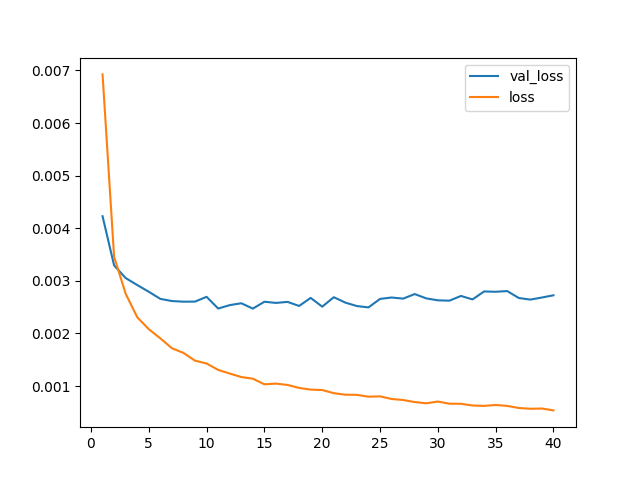
\includegraphics[width=.8\linewidth]{figuras/ape-ajustes-hiper-parametros/cnn-50-k-2.png}
  \caption{Rede convolucional com parâmetro $F = 50$}
  \label{fig:cnn-50-k-2}
\end{subfigure}%
\begin{subfigure}{.5\textwidth}
  \centering
  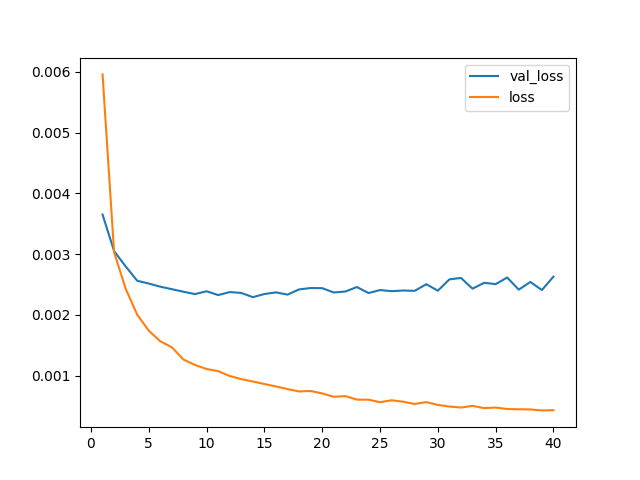
\includegraphics[width=.8\linewidth]{figuras/ape-ajustes-hiper-parametros/cnn-100-k-2.png}
  \caption{Rede convolucional com parâmetro $F = 100$}
  \label{fig:cnn-100-k-2}
\end{subfigure}
\begin{subfigure}{.5\textwidth}
  \centering
  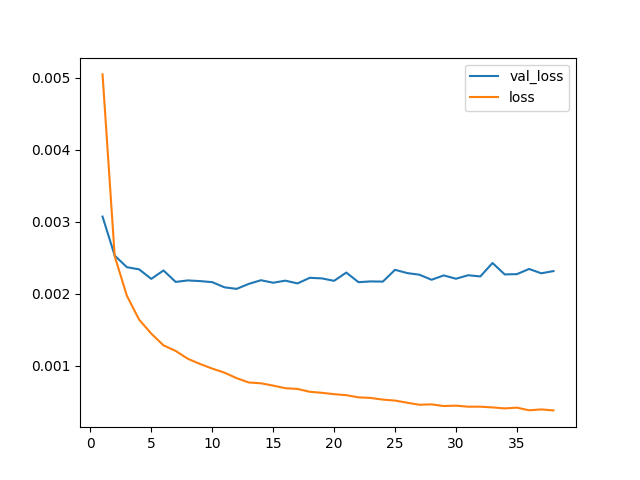
\includegraphics[width=.8\linewidth]{figuras/ape-ajustes-hiper-parametros/cnn-200-k-2.png}
  \caption{Rede convolucional com parâmetro $F = 200$}
  \label{fig:cnn-200-k-2}
\end{subfigure}
\begin{subfigure}{.5\textwidth}
  \centering
  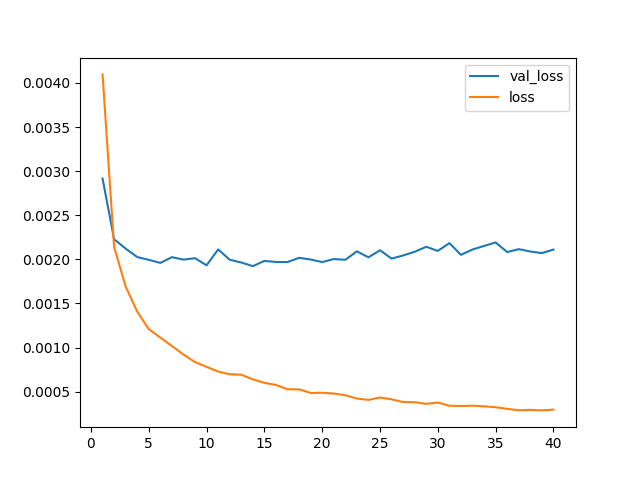
\includegraphics[width=.8\linewidth]{figuras/ape-ajustes-hiper-parametros/cnn-500-k-2.png}
  \caption{Rede convolucional com parâmetro $F = 500$}
  \label{fig:cnn-500-k-2}
\end{subfigure}
\begin{subfigure}{.5\textwidth}
  \centering
  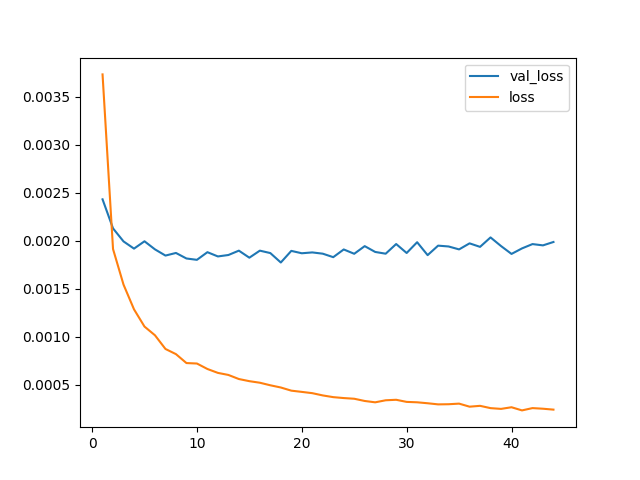
\includegraphics[width=.8\linewidth]{figuras/ape-ajustes-hiper-parametros/cnn-1000-k-2.png}
  \caption{Rede convolucional com parâmetro $F = 1000$}
  \label{fig:cnn-1000-k-2}
\end{subfigure}
\begin{subfigure}{.5\textwidth}
  \centering
  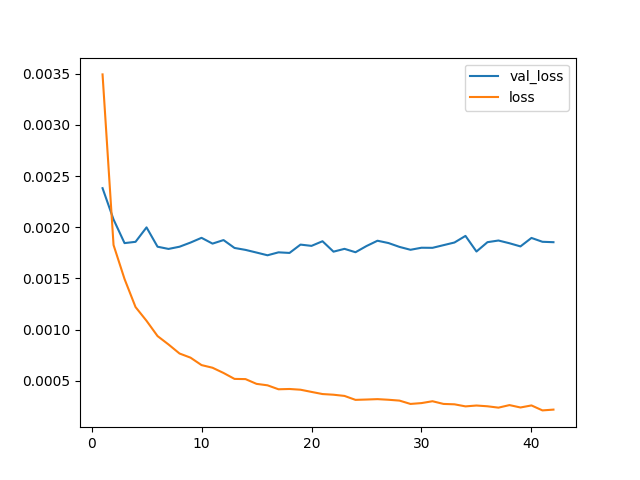
\includegraphics[width=.8\linewidth]{figuras/ape-ajustes-hiper-parametros/cnn-2000-k-2.png}
  \caption{Rede convolucional com parâmetro $F = 2000$}
  \label{fig:cnn-2000-k-2}
\end{subfigure}
\begin{subfigure}{.5\textwidth}
  \centering
  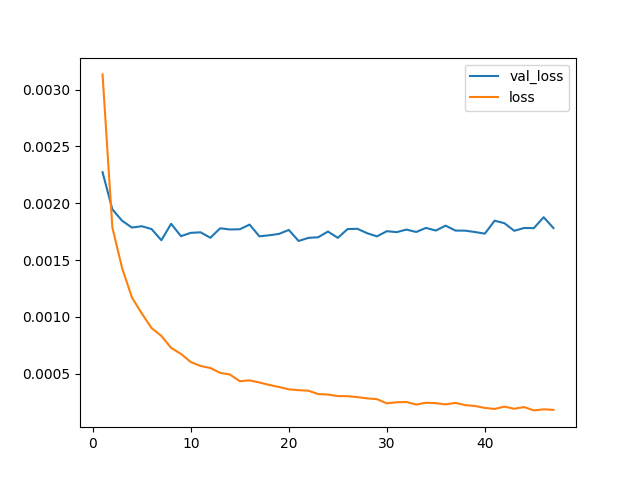
\includegraphics[width=.8\linewidth]{figuras/ape-ajustes-hiper-parametros/cnn-4000-k-2.png}
  \caption{Rede convolucional com parâmetro $F = 4000$}
  \label{fig:cnn-4000-k-2}
\end{subfigure}
\caption{Este gráfico apresenta um comparativo do erro no conjunto de validação em comparação com o erro no conjunto de treinamento. Mais detalhes sobre o treinamento, ver a Seção~\ref{sec:treinamento}. Arquitetura de rede convolucional proposta no Capítulo~\ref{cap:abordagem}, ver Figura~\ref{fig:cnn-architecture}. Hiper-parâmetros: $m = 0.009$, $k = 2$. O parâmetro F indica a quantidade de filtros convolucionais. Nas figuras de \emph{a} a \emph{g}, o eixo \emph{y} indica o valor de erro da função de perda \textit{hinge}, já o eixo \emph{x} indica as épocas de treinamento. A legenda \emph{val\_loss} das figuras de \emph{a} a \emph{g} indica o erro na amostra de validação e a legenda \emph{loss} indica o valor do erro na amostra de treinamento. }
\label{fig:treinamento-cnn-k-2-m-0009}
\end{figure}

De acordo com a Figura~\ref{fig:treinamento-cnn-k-2-m-0009}, o aumento de filtros diminuiu o valor do erro na amostra de validação. O valor de erro que era em torno de $0,003$ na Figura~\ref{fig:cnn-50-k-2}, diminui pela metade, ficando em torno de $0.0015$ nas Figuras~\ref{fig:cnn-2000-k-2} e \ref{fig:cnn-4000-k-2}. O aumento da quantidade de filtros aumenta a capacidade do modelo, pois quanto mais filtros, mais características latentes a rede convolucional tentará extrair dos dados. No nosso caso, isto refletiu no resultado na amostra de validação, diminuindo o valor do erro. Porém, podemos observar que o comportamento do modelo começa a dar sinais de \textit{overfitting}, onde o valor do erro na amostra de treinamento cai abruptamente, enquanto o erro na amostra de validação permance estável e começa a aumentar. Para lidar com este problema, utilizamos normalização em lote e apresentamos os resultados na Seção~\ref{sec:regularizacao-normalizacao-lote}. 

\subsection{Kernel}

Conforme exibido no Capítulo~\ref{cap:abordagem}, o kernel define na rede convolucional de 1 dimensão, o n-grams a serem extraídos. Durante o treinamento, analisamos diferentes valores para o kernel. Verificamos o comportamento para kernel de tamanho 2, 3, 4 e a combinação de valores 2, 3, 5 e 7. Conforme as Figuras~\ref{fig:treinamento-cnn-diferentes-kernels} e \ref{fig:treinamento-cnn-diferentes-kernels-2}, não houve melhora significativa para kernels de tamanho 3 e 4 em comparação com o kernel de tamanho 2. E até mesmo a combinação de kernels não gerou uma melhora significativa dado a quantidade de parâmetros utilizados. Neste caso, optamos por manter o kernel fixado em $2$.


\begin{figure}[H]
\begin{subfigure}{.5\textwidth}
  \centering
  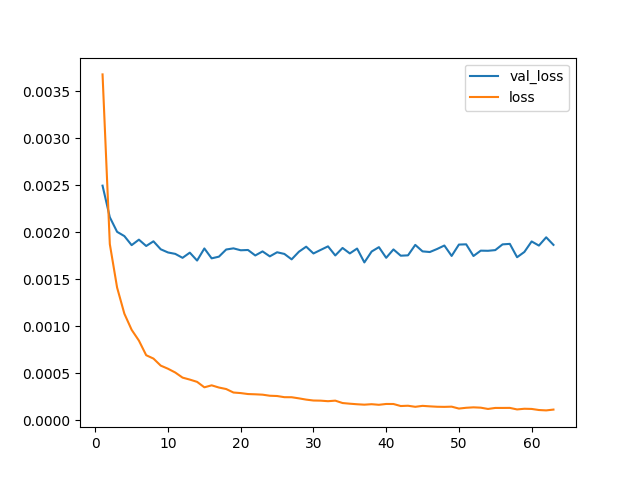
\includegraphics[width=.8\linewidth]{figuras/ape-ajustes-hiper-parametros/cnn-1000.png}
  \caption{Rede convolucional com parâmetro $F = 1000$ e $K = [2,3,5,7]$}
  \label{fig:cnn-1000}
\end{subfigure}%
\begin{subfigure}{.5\textwidth}
  \centering
  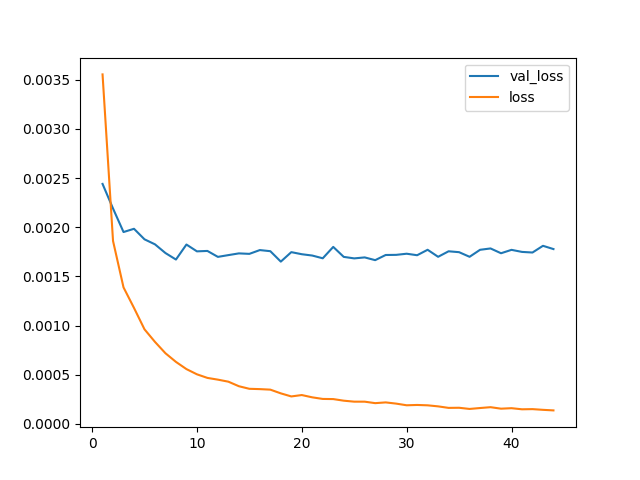
\includegraphics[width=.8\linewidth]{figuras/ape-ajustes-hiper-parametros/cnn-2000.png}
  \caption{Rede convolucional com parâmetro $F = 2000$ e $K = [2, 3, 5, 7]$}
  \label{fig:cnn-2000}
\end{subfigure}
\begin{subfigure}{.5\textwidth}
  \centering
  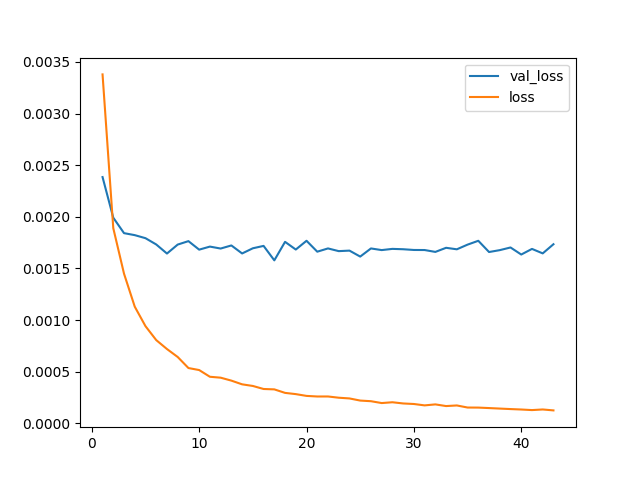
\includegraphics[width=.8\linewidth]{figuras/ape-ajustes-hiper-parametros/cnn-4000.png}
  \caption{Rede convolucional com parâmetro $F = 4000$ e $K = [2, 3, 5, 7]$}
  \label{fig:cnn-4000}
\end{subfigure}
\begin{subfigure}{.5\textwidth}
  \centering
  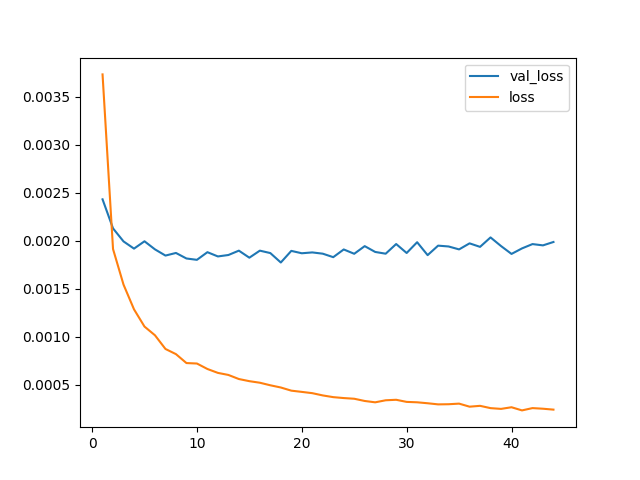
\includegraphics[width=.8\linewidth]{figuras/ape-ajustes-hiper-parametros/cnn-1000-k-2.png}
  \caption{Rede convolucional com parâmetro $F = 1000$ e $K = 2$}
  \label{fig:cnn-1000-k-2-v2}
\end{subfigure}
\begin{subfigure}{.5\textwidth}
  \centering
  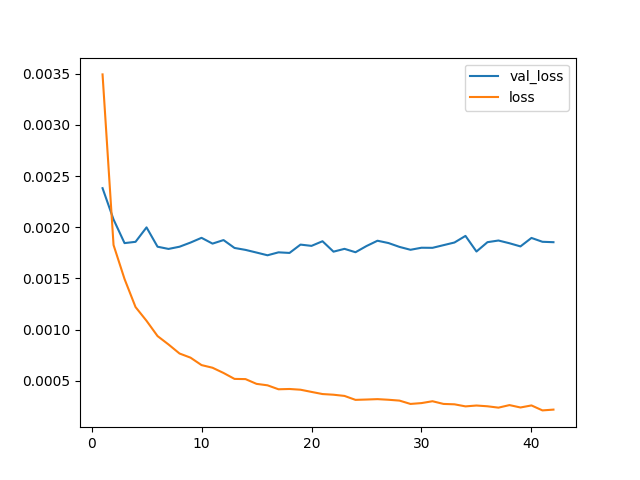
\includegraphics[width=.8\linewidth]{figuras/ape-ajustes-hiper-parametros/cnn-2000-k-2.png}
  \caption{Rede convolucional com parâmetro $F = 2000$ e $K = 2$}
  \label{fig:cnn-2000-k-2-v2}
\end{subfigure}
\begin{subfigure}{.5\textwidth}
  \centering
  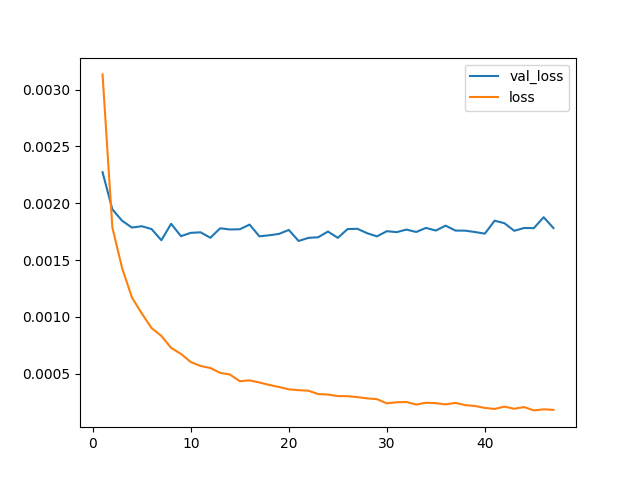
\includegraphics[width=.8\linewidth]{figuras/ape-ajustes-hiper-parametros/cnn-4000-k-2.png}
  \caption{Rede convolucional com parâmetro $F = 4000$ e $K = 2$}
  \label{fig:cnn-4000-k-2-v2}
\end{subfigure}
\caption{Gráfico do treinamento da rede convolucional na recuperação de trecho de código-fonte. Este gráfico apresenta um comparativo do erro no conjunto de validação em comparação com o erro no conjunto de treinamento. Mais detalhes sobre o treinamento, ver a Seção~\ref{sec:treinamento}. Arquitetura de rede convolucional proposta no Capítulo~\ref{cap:abordagem}, ver Figura~\ref{fig:cnn-architecture}. Hiper-parâmetros: $m = 0.009$. O parâmetro F indica a quantidade de filtros convolucionais, o parâmetro K indica o tamanho da janela do filtro convolucional. Nas figuras de \emph{a} a \emph{f}, o eixo \emph{y} indica o valor de erro da função de perda \textit{hinge}, já o eixo \emph{x} indica as épocas de treinamento. A legenda \emph{val\_loss} das figuras de \emph{a} a \emph{g} indica o erro na amostra de validação e a legenda \emph{loss} indica o valor do erro na amostra de treinamento. }
\label{fig:treinamento-cnn-diferentes-kernels}
\end{figure}

\begin{figure}[H]
\begin{subfigure}{.5\textwidth}
  \centering
  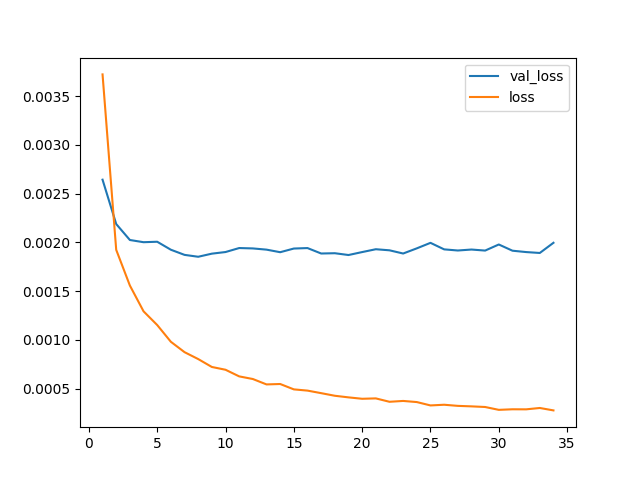
\includegraphics[width=.8\linewidth]{figuras/ape-ajustes-hiper-parametros/cnn-1000-k-3.png}
  \caption{Rede convolucional com parâmetro $F = 1000$ e $K = 3$}
  \label{fig:cnn-1000-k-3}
\end{subfigure}
\begin{subfigure}{.5\textwidth}
  \centering
  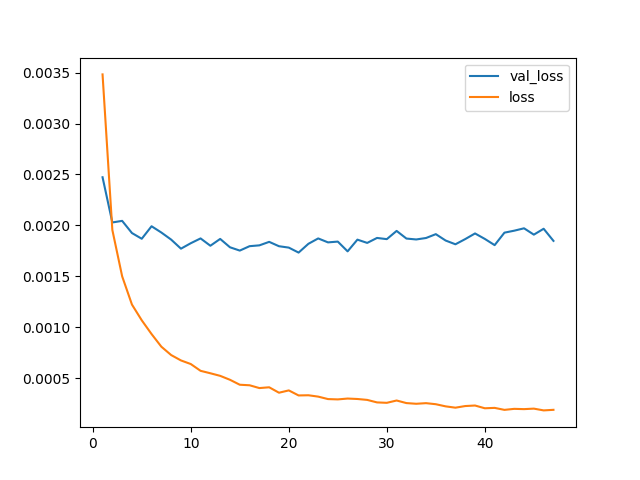
\includegraphics[width=.8\linewidth]{figuras/ape-ajustes-hiper-parametros/cnn-2000-k-3.png}
  \caption{Rede convolucional com parâmetro $F = 2000$ e $K = 3$}
  \label{fig:cnn-2000-k-3}
\end{subfigure}
\begin{subfigure}{.5\textwidth}
  \centering
  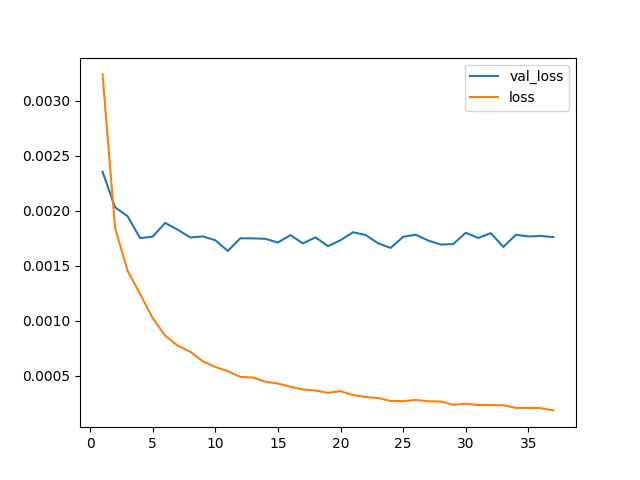
\includegraphics[width=.8\linewidth]{figuras/ape-ajustes-hiper-parametros/cnn-4000-k-3.png}
  \caption{Rede convolucional com parâmetro $F = 4000$ e $K = 3$}
  \label{fig:cnn-4000-k-3}
\end{subfigure}
\begin{subfigure}{.5\textwidth}
  \centering
  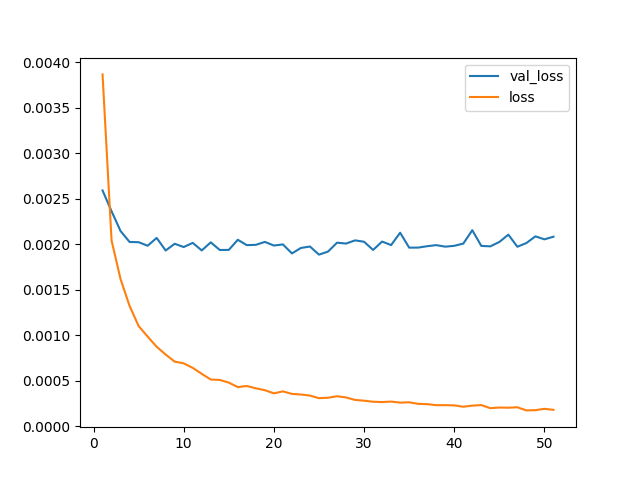
\includegraphics[width=.8\linewidth]{figuras/ape-ajustes-hiper-parametros/cnn-1000-k-4.png}
  \caption{Rede convolucional com parâmetro $F = 1000$ e $K = 4$}
  \label{fig:cnn-1000-k-4}
\end{subfigure}
\begin{subfigure}{.5\textwidth}
  \centering
  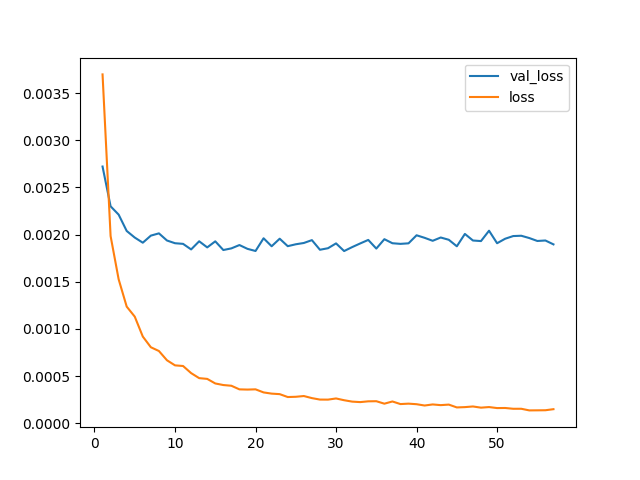
\includegraphics[width=.8\linewidth]{figuras/ape-ajustes-hiper-parametros/cnn-2000-k-4.png}
  \caption{Rede convolucional com parâmetro $F = 2000$ e $K = 4$}
  \label{fig:cnn-2000-k-4}
\end{subfigure}
\begin{subfigure}{.5\textwidth}
  \centering
  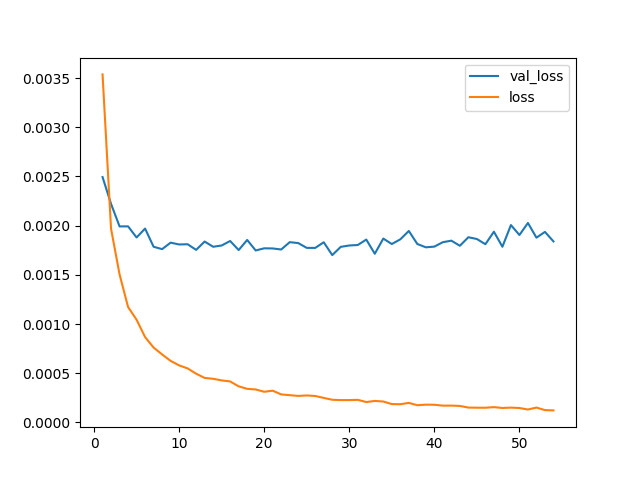
\includegraphics[width=.8\linewidth]{figuras/ape-ajustes-hiper-parametros/cnn-4000-k-4.png}
  \caption{Rede convolucional com parâmetro $F = 4000$ e $K = 4$}
  \label{fig:cnn-4000-k-4}
\end{subfigure}
\caption{Gráfico do treinamento da rede convolucional na recuperação de trecho de código-fonte. Este gráfico apresenta um comparativo do erro no conjunto de validação em comparação com o erro no conjunto de treinamento. Mais detalhes sobre o treinamento, ver a Seção~\ref{sec:treinamento}. Arquitetura de rede convolucional proposta no Capítulo~\ref{cap:abordagem}, ver Figura~\ref{fig:cnn-architecture}. Hiper-parâmetros: $m = 0.009$. O parâmetro F indica a quantidade de filtros convolucionais, o parâmetro K indica o tamanho da janela do filtro convolucional. Nas figuras de \emph{a} a \emph{f}, o eixo \emph{y} indica o valor de erro da função de perda \textit{hinge}, já o eixo \emph{x} indica as épocas de treinamento. A legenda \emph{val\_loss} das figuras de \emph{a} a \emph{g} indica o erro na amostra de validação e a legenda \emph{loss} indica o valor do erro na amostra de treinamento. }
\label{fig:treinamento-cnn-diferentes-kernels-2}
\end{figure}



\section{Ajuste da margem - Função de perda hinge}

Além dos hiper-parâmetros das redes convolucionais, a função de perda \textit{hinge} conforme descrito na Seção~\ref{sec:funcao-objetivo}, exige um parâmetro \emph{margem}. Este parâmetro define a magnitude da diferença da distância de similaridade entre os trechos de código anotados como corretos e os trechos que não são respostas com relação às questões. Os pesquisadores \cite{feng-2015} recomendaram uma margem de $0,009$, enquanto \cite{tan-lstm-qa} utilizaram uma margem de $0,2$. Em nosso caso, fizemos alguns experimentos com os valores $0,009$, $0,05$, $0,1$ e $0,2$. 


\begin{table}[H]
\centering
\begin{tabular}{ p{1cm} p{4cm} P{2.2cm} P{2.2cm} P{2.2cm} P{2.2cm} }
 \hline
    & & \multicolumn{4}{c}{\textbf{Resultados MRR}}\\
 \hline
 & \textbf{Modelos} & \textbf{$m = 0,009$} & \textbf{$m = 0,05$} & \textbf{$m = 0,1$}& \textbf{$m = 0,2$}\\
 \hline
 A1 & Embedding & $0.600$& $0.632$& \cellcolor{Gray!35} $0.637$& $0.635$\\
 
 \hline
 \
 B1 & Unif & $0.647 $ & $0.652$& $0.660$& \cellcolor{Gray!35} $0.674$\\
 
 \hline
 
 C1 & CNN / F = 1000 & $0.654 $ & $0.669$& \cellcolor{Gray!35} $0.676$& $0.637$\\
 
 C2 & CNN / F = 2000 & $0.675 $ & \cellcolor{Gray!35} $0.673$& $0.661$& $0.647$\\
 
 C3 & CNN / F = 4000 & $0.664$ & \cellcolor{Gray!35} $0.687$& $0.672$& $0.651$\\
 
\hline
\end{tabular}
\caption{Resultado da avaliação dos modelos CNN, \Gls{unif} e Embedding na amostra EVAL. MRR refere-se a média do resultado do Mean Reciprocal Rank (equação~\ref{eq:mrr}). O hiper-parâmetro \emph{m} indica a margem utilizada na função de perda \textit{hinge}. F indica a quantidade de filtros convolucionais utilizados durante o treinamento das redes convolucionais. As células destacadas indicam a margem na qual o modelo obteve o melhor desempenho durante a avaliação.}
\label{table:alteracao-margem}
\end{table}



Notamos que não há um consenso sobre o valor da margem, conforme a Tabela~\ref{table:alteracao-margem}, cada arquitetura obteve um melhor desempenho para um valor diferente de margem. As redes convolucionais obtiveram o melhor desempenho para uma margem de valor $0,05$, exceto quando a quantidade de filtros convolucionais utilizadas é $1000$. Já a arquitetura Unif proposta por \cite{cambronero-deep-learning-code-search:2019} obteve o melhor desempenho para o valor $0,2$, enquanto a arquitetura \textit{Embedding} obteve com o valor $0,1$. Optamos por fixar estes valores específicos para cada arquitetura, então no caso do CNN fixamos a margem em $0,5$, enquanto para Unif e \textit{Embedding} fixamos em $0,2$ e $0,1$ respectivamente. E conforme descrito na Tabela~\ref{table:alteracao-margem}, escolhemos o valor da margem baseado no valor mais alto da métrica MRR, que foi obtida através da avaliação do melhor modelo na amostra EVAL. Ver a Seção~\ref{sec:avaliacao} para mais detalhes sobre o procedimento de avaliação. 

\section{Regularização - Normalização em Lote}
\label{sec:regularizacao-normalizacao-lote}

Conforme as Figuras~\ref{fig:cnn-1000-k-2-v2}, \ref{fig:cnn-2000-k-2-v2} e \ref{fig:cnn-4000-k-2-v2}, as redes convolucionais estão dando sinais de \textit{overfitting}, onde o valor do erro na amostra de treinamento está diminuindo rapidamente, enquanto o valor do erro na amostra de validação está estável e aumentando ao longo do tempo. Para tentar redimir este problema, aplicamos a normalização em lote para regularizar o nosso modelo. Conforme \cite{sergey-batch-normalization-2015}, a aprendizagem em redes neurais profundas é complicada, pois a distribuição de cada camada é alterada, conforme os parâmetros são atualizados ao longo do treinamento. Isto requer uma otimização e ajuste dos parâmetros a fim de evitar a saturação da função de perda. Para mitigar este problema e auxiliar o modelo a aprender de maneira mais rápida, os pesquisadores apresentaram a normalização em lote, que permite utilizarmos taxas de aprendizagem mais alta e não requer muitos cuidados na inicialização do modelo. Além disso, segundo os próprios pesquisadores, a normalização em lote além de ajudar o modelo a aprender mais rápido, ela auxiliou na melhora do desempenho e obtenção de um modelo mais robusto, não necessitando de outras técnicas de regularização como \textit{dropout} \citep{sergey-batch-normalization-2015}.

Aplicamos a normalização em lote nas redes convolucioanais e também na arquitetura Unif proposta por \cite{cambronero-deep-learning-code-search:2019}. Conforme as Figuras XXXXX, podemos notar uma melhora na aprendizagem com a normalização em lote e uma melhora no desempenho para as redes convolucionais. No caso da arquitetura Unif, não notamos diferença no desempenho. E optamos por apresentar ambos os resultados na Seção~\ref{table:resultados}. 





%\chapter{Sequências}
\label{ape:sequencias}

Texto texto texto texto texto texto texto texto texto texto texto texto texto
texto texto texto texto texto texto texto texto texto texto texto texto texto
texto texto texto texto texto texto.


\singlespacing

\renewcommand{\arraystretch}{0.85}
\captionsetup{margin=1.0cm}  % corre?o nas margens dos captions.
%--------------------------------------------------------------------------------------
\begin{table}
\begin{center}
\begin{small}
\begin{tabular}{|c|c|c|c|c|c|c|c|c|c|c|c|c|} 
\hline
\emph{Limiar} & 
\multicolumn{3}{c|}{MGWT} & 
\multicolumn{3}{c|}{AMI} &  
\multicolumn{3}{c|}{\emph{Spectrum} de Fourier} & 
\multicolumn{3}{c|}{Características espectrais} \\
\cline{2-4} \cline{5-7} \cline{8-10} \cline{11-13} & 
\emph{Sn} & \emph{Sp} & \emph{AC} & 
\emph{Sn} & \emph{Sp} & \emph{AC} & 
\emph{Sn} & \emph{Sp} & \emph{AC} & 
\emph{Sn} & \emph{Sp} & \emph{AC}\\ \hline \hline
 1 & 1.00 & 0.16 & 0.08 & 1.00 & 0.16 & 0.08 & 1.00 & 0.16 & 0.08 & 1.00 & 0.16 & 0.08 \\
 2 & 1.00 & 0.16 & 0.09 & 1.00 & 0.16 & 0.09 & 1.00 & 0.16 & 0.09 & 1.00 & 0.16 & 0.09 \\
 2 & 1.00 & 0.16 & 0.10 & 1.00 & 0.16 & 0.10 & 1.00 & 0.16 & 0.10 & 1.00 & 0.16 & 0.10 \\
 4 & 1.00 & 0.16 & 0.10 & 1.00 & 0.16 & 0.10 & 1.00 & 0.16 & 0.10 & 1.00 & 0.16 & 0.10 \\
 5 & 1.00 & 0.16 & 0.11 & 1.00 & 0.16 & 0.11 & 1.00 & 0.16 & 0.11 & 1.00 & 0.16 & 0.11 \\
 6 & 1.00 & 0.16 & 0.12 & 1.00 & 0.16 & 0.12 & 1.00 & 0.16 & 0.12 & 1.00 & 0.16 & 0.12 \\
 7 & 1.00 & 0.17 & 0.12 & 1.00 & 0.17 & 0.12 & 1.00 & 0.17 & 0.12 & 1.00 & 0.17 & 0.13 \\
 8 & 1.00 & 0.17 & 0.13 & 1.00 & 0.17 & 0.13 & 1.00 & 0.17 & 0.13 & 1.00 & 0.17 & 0.13 \\
 9 & 1.00 & 0.17 & 0.14 & 1.00 & 0.17 & 0.14 & 1.00 & 0.17 & 0.14 & 1.00 & 0.17 & 0.14 \\
10 & 1.00 & 0.17 & 0.15 & 1.00 & 0.17 & 0.15 & 1.00 & 0.17 & 0.15 & 1.00 & 0.17 & 0.15 \\
11 & 1.00 & 0.17 & 0.15 & 1.00 & 0.17 & 0.15 & 1.00 & 0.17 & 0.15 & 1.00 & 0.17 & 0.15 \\
12 & 1.00 & 0.18 & 0.16 & 1.00 & 0.18 & 0.16 & 1.00 & 0.18 & 0.16 & 1.00 & 0.18 & 0.16 \\
13 & 1.00 & 0.18 & 0.17 & 1.00 & 0.18 & 0.17 & 1.00 & 0.18 & 0.17 & 1.00 & 0.18 & 0.17 \\
14 & 1.00 & 0.18 & 0.17 & 1.00 & 0.18 & 0.17 & 1.00 & 0.18 & 0.17 & 1.00 & 0.18 & 0.17 \\
15 & 1.00 & 0.18 & 0.18 & 1.00 & 0.18 & 0.18 & 1.00 & 0.18 & 0.18 & 1.00 & 0.18 & 0.18 \\
16 & 1.00 & 0.18 & 0.19 & 1.00 & 0.18 & 0.19 & 1.00 & 0.18 & 0.19 & 1.00 & 0.18 & 0.19 \\
17 & 1.00 & 0.19 & 0.19 & 1.00 & 0.19 & 0.19 & 1.00 & 0.19 & 0.19 & 1.00 & 0.19 & 0.19 \\
17 & 1.00 & 0.19 & 0.20 & 1.00 & 0.19 & 0.20 & 1.00 & 0.19 & 0.20 & 1.00 & 0.19 & 0.20 \\
19 & 1.00 & 0.19 & 0.21 & 1.00 & 0.19 & 0.21 & 1.00 & 0.19 & 0.21 & 1.00 & 0.19 & 0.21 \\
20 & 1.00 & 0.19 & 0.22 & 1.00 & 0.19 & 0.22 & 1.00 & 0.19 & 0.22 & 1.00 & 0.19 & 0.22 \\ \hline 
\end{tabular}
\caption{Exemplo de tabela.}
\label{tab:tab:F5}
\end{small}
\end{center}
\end{table}

      % associado ao arquivo: 'ape-conjuntos.tex'

% ---------------------------------------------------------------------------- %
% Bibliografia
\backmatter \doublespacing   % espa?mento duplo
\bibliographystyle{plainnat-ime} % cita?o bibliogr?ica textual
\bibliography{bibliografia}  % associado ao arquivo: 'bibliografia.bib'

% ---------------------------------------------------------------------------- %
% ?dice remissivo
% \index{TBP|see{periodicidade região codificante}}
% \index{DSP|see{processamento digital de sinais}}
% \index{STFT|see{transformada de Fourier de tempo reduzido}}
% \index{DFT|see{transformada discreta de Fourier}}
% \index{Fourier!transformada|see{transformada de Fourier}}

% \printindex   % imprime o ?dice remissivo no documento 

\end{document}
